\documentclass[senior]{IPSstyle}

  \Year{2017}
  \Month{February}
  \Author{44151568-7: Wei CAO}

  \Title{Stacked Residual Recurrent Neural Network with Word Weight for Text Classification}

  \Advisor{Professor Jinglu HU}

\usepackage{amssymb,amsmath}

\usepackage{mathptmx}
\usepackage{helvet}
\usepackage{courier}
\usepackage{type1cm}

\usepackage{makeidx}
\usepackage{graphicx,subfigure}
\usepackage{multicol}
\usepackage{multirow}
\usepackage[bottom]{footmisc}

\usepackage{mathrsfs}
\usepackage{amssymb,amsmath}
\usepackage{amsfonts}
\usepackage{color}
\usepackage{CJKutf8}

\usepackage{listings}
\usepackage{algorithm,algorithmicx,algpseudocode}
\usepackage[toc,page,title,titletoc,header]{appendix}

\renewcommand{\algorithmicrequire}{\textbf{Input:}}
\renewcommand{\algorithmicensure}{\textbf{Output:}}

  \Abstract{
Neural networks, and in particular recurrent neural networks (RNNs) have recently been shown to give a state-of-the-art performance on some text classification tasks. However, most existing methods assume that each word in a sentence contributes the same importance, it is different from the real world. For example, if we do sentiment analysis, the word "awesome" is much more importance than any other words in sentence "This movie is awesome". Motivated by this deficiency and in order to achieve a further performance, in this paper, a Stacked Residual RNN with Word Weight method is proposed, we extend the stacked RNN networks to a deep one with residual network architecture and introduce a word weight network. Our proposed method is able to learn high hierarchical meaning of each word in a sentence and consider the weight of each word for text classification task. Experimental result indicates that our method achieves high performance and it can get state-of-art result on two text classification tasks.

}

\Keywords{Recurrent Neural Networks, Text Classification, Deep Learning, Long Short-Term Memory}

\Acknowledgments{
   It is quite unforgetable time I spend in here, Furuzuki Lab, Waseda University. I would like deeply thank to my professor, Jinglu HU for guiding me in my research. In the last one and a half years, he has provided me insightful advice, patient guidance, and enough independence. Professor HU always give helpful and appropriate suggestions on how to handle those problems with his breadth of mind.

   I extend my warmest thanks to my professor Anping SONG in Shanghai University, who recommends me to Waseda University and gives me great support to complete my study in Japan, which is an amazing life experience.

   Thanks all my friends and families for your great support and companion, this paper can not be finished without your patient to comfort me.



}


\begin{document}

 \makepreliminarypages
 \singlespace
 \frontmatter
 \tableofcontents
 \listoffigures
 \listoftables
 \mainmatter
 \clearemptydoublepage
 \setlength{\baselineskip}{23.0pt}

\chapter{Introduction}



\section{Background and Motivation}

Text classification is one of the main research areas in natural language processing, in which one needs to assign a label to each sentence. It has been widely used in some applications including sentiment analysis\cite{maas2011learning}\cite{ghiassi2013twitter}, question type classification\cite{zhang2003question}\cite{li2002learning}and topic type labeling\cite{wang2012baselines}\cite{quercia2012tweetlda}.

Sentence modeling is an important step as a core step in natural language processing for representing phrases and sentences into meaningful feature vectors. There are three main methods for sentence modeling which are: bag-of-words models, sequence based models and tree-structured models. The traditional way for sentence modeling is based on bag-of-words which do not consider the order of words. For example, each phrases and sentences can be represented by frequency of each word in corpus\cite{joachims2002statistical}\cite{joachims1998text}. In sequence based models, it considers the ordered sequence of tokens for its representation\cite{mikolov2010recurrent}\cite{johnson2014effective}. Tree structured models construct each word into a syntactic tree over the sentence\cite{socher2013recursive}.

Recurrent neural network (RNN)\cite{elman1990finding} is an effective tool for sequence modeling tasks. RNNs with Long Short-Term Memory (LSTM) structure\cite{hochreiter1997long} has a modified hidden state update which can more effectively capture long-term dependencies. LSTMs has been widely used in many sequence modeling and prediction tasks, especially speech recognition\cite{li2015constructing}, handwriting recognition\cite{breuel2013high}, and machine translation\cite{sutskever2014sequence}.

Although recurrent neural networks based classifiers can get high performance in many text classification\cite{lee2016sequential}\cite{zhou2015end}, these neural text classification models do not consider the different importance of each word in a sentence. For instance, in sentence “Today is so great”, the word “great” is much more important than other words in sentiment analysis task,  another example is that the word "awesome" is much more importance than any other words in sentence "This movie is awesome".

Residual networks\cite{he2015deep} is an intriguing network which can overcome the disadvantage of vanishing gradients, exploding gradients and difficulties during the training process due to the increasing network depth in image recognition task.

Inspired by the high performance of residual networks for training deep neural networks and in order to overcome the deficiency of ignoring the contribution of different word in standard recurrent neural networks, in this paper, we propose a stacked RNNs model which is based on word weight and residual networks. In this model, “word weight” part of network can consider the different contribution of words in a sentence, “residual learning” part of network can improve the performance of stacked recurrent neural networks. We evaluate our model on three experiment of two datasets, our proposed method is able to learn high hierarchical meaning of each word in a sentence and consider the weight of each word for text classification task, the experiment results show that our model outperforms the existing systems.


%%%%%%%%%%%%%%%%%%%%%%%%%%%%%%%%%%%%%%%%%%%%%%%%%%%%%%%%%%%%%%%%%%%%%%%%%%%%%%%


\section{Organization of the thesis}
The remainder of this thesis is structured as follows: Chapter \uppercase\expandafter{\romannumeral2}  introduces some related works in the field of text classification and describes some commonly model in this area. In Chapter \uppercase\expandafter{\romannumeral3}, we describe the proposed method, which describe the structure and mechanism of Stacked Residual Bi-LSTM with Word Weight model. To evaluate the proposed method and testify its effectiveness, Chapter \uppercase\expandafter{\romannumeral4} evaluates our model on three text classification tasks. The thesis ends in Chapter \uppercase\expandafter{\romannumeral5} with conclusions on contributions of this work.

%%%%%%%%%%%%%%%%%%%%%%%%%%%%%%%%%%%%%%%%%%%%%%%%%%%%%%%%%%%%%%Chapter 3
\chapter{Related Work} \label{ch3}
%%%%%%%%%%%%%%%%%%%%%%%%%%%%%%%%%%%%%%%%%%%%%%%%%%%%%%%%%%%%%%Chapter 3



%%%%%%%%%%%%%%%%%%%%%%%%%%%%%%%%%%%%%%%%%%%%%%%%%%%%%%%%%%%%%%%%%%%%%%%%%%%%%%%
With the growth of Web information, textual data gains increasingly high importances.  People largely  access  information  from  these  online textual data sources rather than being limited to archaic paper sources like books, magazines etc. But  the  the biggest  problem  is  that  this  information  lacks  organization  which  makes  it difficult  to  search and manage.  Text  classification  is  one  of  the  efficient techniques  used  for organizing such kind of digital data.  

The  aim  of  text  classification task  is to  build  systems  which are able  to automatically
classify  documents  into labels based  on  their  content. A supervised classification algorithm allows us to access the data labels during the training and testing steps. In this section, we provides a review of some related works of generic text classification methods which use machine learning algorithms for text classification task.


\section{Traditional related methods}

Most of traditional related methods focus on how to build a powerful classifier, these algorithms try to modify structure of classifier rather than extract more features in classification task. In feature extraction step, they often use some common methods, the most common method is word frequency distribution which is the bag-of-word based method. In preparation for the feature extraction, the algorithm would look at all available texts and count the frequency of each word that occurs in these texts. Each word in the vector is then allocated a dimension in the feature vector.  When feature vector of a text is extracted, each value in the feature vector will represent the number of times each word has occurred in the text.

\begin{figure}[t]
  \centering
  % Requires \usepackage{graphicx}
  \includegraphics[width=10cm]{word_distribution.png}\\
  \caption{An illustration of feature extraction.}\label{NBde}
\end{figure}

\subsection{Support Vector Machines based methods}

Support Vector Machine (SVM) is one of the discriminative classification method. It is a supervised machine learning algorithm which can be used for  text classification. The idea of SVM is based on structural risk minimization theory\cite{vapnik2013nature}. SVM tries to use linear or non-linear delineations between the different classes to partition the data space. The most important thing in such classifiers is to find the optimal boundaries between the different classes and use them for the classification task.

\begin{figure}[t]
  \centering
  % Requires \usepackage{graphicx}
  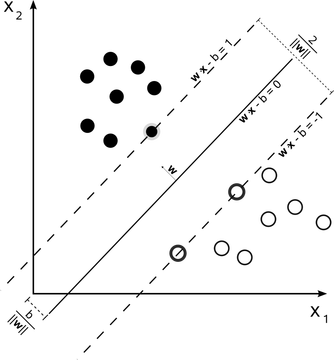
\includegraphics[width=9cm]{svm.png}\\
  \caption{An illustration of SVM for choosing the hypeplane that maximizes the margin in 2D-space.}\label{NBde}
\end{figure}

In the Figure 2.1, we can see this illustrated for the example data in 2D-space. The points which display in figure are labeled  with two different color. SVM finds the hypeplane that can maximizes the margin between the two labels. This hyperplane is given as follow:
\begin{equation}
\left \langle \vec{w} \cdot \vec{x} \right \rangle + b = \sum_{i=1}^N y_i \alpha_i \left \langle \vec{x_i} \cdot \vec{x} \right \rangle + b = 0
\end{equation}
where $\vec{x_i}=(x_{i1},x_{i2},...x_{in})$ is a input vector which has n-dimensional , $y_i$ is  output data, $\vec{w}=(w_{1},w_{2},...w_{n})$ is the weight vector which defines the hyperplane and the $\alpha+i$ terms are the Lagrangian multipliers.

Once the hyperplane is constructed  in training data, the class of test data $\vec{x_i}$ can be determined as follow:
if $\vec{w} \cdot \vec{x_i} + b \geq 0$ then it belongs to the label 0, if $\vec{w} \cdot \vec{x_i} + b \leq 0$ then it belongs to the label 1.

\subsection{Naive Bayes based methods:}

Naive Bayes classifier is a classical classification algorithm which is based on Bayes theorem with strong and naive independence assumptions.  Bayesian classifier is the simplest with it's linear classifiers, but it is still very effective. Naive Bayes classifier assumes that the features of
the input feature vector (word distribution) which were used in the classification are statistically independent\cite{brucher2002document}. In a text classification problem, the idea of Naive Bayes classifier is to classify text by using the posterior probability of the texts which belong to the different classes. The probability of a class $C$ is given by the posterior probability $P(C|D)$ given a training data $D$. Here $D$ refers to all of the text in the entire training data. It is given by $D=(d_1, d_2,...d_n)$, where $d_i$ is the $i_{th}$ attribute (word) of document $D$.

In Bayes' rule, the posterior probability is as follow:
\begin{equation}
P(C=c_i | D) = \frac{P(D | C=c_i) \cdot P(C=c_i)}{P(D)}
\end{equation}

$P(D)$ is equal for all classes, it can be disregarded and the equation can change to:
\begin{equation}
P(C=c_i | D) = P(D | C=c_i) \cdot P(C=c_i)
\end{equation}

The document D belongs to the class C which would maximizes this probability:
\begin{equation}
\begin{split}
C &= argmax P(D|C) \cdot P(C) \\
& = argmax P(d_1, d_2, ..,d_n|C) \cdot P(C)
\end{split}
\end{equation}

Then, we assume that each words $d_i$ is conditional independent and the equation can change to:
\begin{equation}
\begin{split}
C &= argmax P(d_1|C) \cdot P(d_2|C) \cdot \cdot \cdot P(d_n|C) \cdot P(C) \\
& = argmax \prod_{i=1}^{n} P(d_i|C) \cdot P(C)
\end{split}
\end{equation}
where $P(d_i | C)$ is the conditional probability that word $i$ belongs to class $C$ which can be calculated as below:
\begin{equation}
P(d_i | C) = \frac{count(d_i, C)}{\sum_i count(d_i, C)}
\end{equation}

\subsection{k Nearest Neighbours based methods:}

\begin{figure}[t]
  \centering
  % Requires \usepackage{graphicx}
  \includegraphics[width=9cm]{knn.png}\\
  \caption{An illustration of k-Nearest Neighbor.}\label{NBde}
\end{figure}

k Nearest Neighbours (kNN) classifier is one of the simplest geometrical classifiers\cite{kwon2003text}.  The  kNN  method  is  outstanding  with  its  simplicity and is widely used techniques for text classification.  This  method  performs  well  even  in  handling  the classification   tasks   with   multi-label   documents.   

The basic idea of kNN is very simple, it  is used  to  test  the  degree  of  similarity  between  documents  and  k   training  data  and  to  store  a  certain  amount  of  classification  data. In the high dimension space, each document can be seen as a point in it which represents the document being classified. Each test data has it's own position and there are too many others points around this it, but only k number of nearest neighbours are considered. If these data belong to the same label then the new document also will be classified to that label. This method is an instant-based learning algorithm that classified objects based on closest feature space in the  training  set.

On the other hand, the accuracy of kNN  is  severely  degraded  by  the  data noisy  and  irrelevant features. 



\subsection{Decision Trees based methods:}

Decision trees are hierarchical model for supervised learning with the underlying data space by using the different text features. The  decision  tree  rebuilds  the  manual  class  of  training     data     by     constructing     well-defined   true or false conditional queries in the form of a tree structure. It is composed with the internal decision nodes and terminal leaves. The internal nodes are labeled by the features and the leaves are labeled by classes.  The well-trained decision tree can  classify a document by  scanning it in the root node of the tree and judging through 
the  conditional query  structure  until  it  reaches  to leaf node easily,  this leaf node would   represents the classification of the document. 

\begin{figure}[t]
  \centering
  % Requires \usepackage{graphicx}
  \includegraphics[width=9cm]{tree.png}\\
  \caption{An illustration of Decision trees.}\label{NBde}
\end{figure}


%%%%%%%%%%%%%%%%%%%%%%%%%%%%%%%%%%%%%%%%%%%%%%%%%%%%%%%%%%%%%%%%%%%%%%%%%%%%%%%

\begin{figure}[t]
  \centering
  % Requires \usepackage{graphicx}
  \includegraphics[width=9cm]{ann.png}\\
  \caption{An illustration of simple Neural Netowrks.}\label{NBde}
\end{figure}

\section{Neural Networks related methods}

Neural Network is a massively parallel distributed network which is consist of  a large number of simple artificial neurons, these neurons are able to learn knowledge from experience during the training and making it available for use. These artificial  neurons  are  interconnected into  group  using  a  mathematical model for information processing. Neural Network is try to simulated human brain which may contains hundreds of thousands or even millions of parameters, the strong neural network can be seen as an "expert" in specific area such as text classification task.

Different from the traditional related method, Neural Networks related method in classification task is focus on how to extract high hierarchical features from data rather than build a powerful classifier. No matter how complicated the network is, it always used to extract feature vectors in previous layers, the classifier of last layer is often use Softmax. 

There are too many different  types  of  Neural  Network  methods  have  been  applied  to  text  classification  tasks. Generally speaking,  Neural  Network for any classification task is as follow: a Neural  Network is taken, data of the feature vector is fed to the inputs of the network and the label of data comes from the outputs.

With the growth depth of neural network, GPU become more and more important in deep learning area because of it's high computation usage. Deep learning based methods have achieved high performance on text classification tasks. Too many researchers have devoted themselves into  deep learning based research area for text classification  in recent years. Le et al. (2014) \cite{le2014distributed} proposed the Paragraph Vector method for representations of sentences and documents. Zhang et al. (2015) \cite{zhang2015character} constructed a Character-level Convolutional Networks for doing text classification. Kim et al. (2014) \cite{kim2014convolutional} proposed a Convolutional Neural Networks for Sentence Classification which consider each words as n-gram to do embedding operation. Johnson et al. (2015) \cite{johnson2015semi} proposed a scheme for embedding learning of small text regions which is based on the idea of two-view semi-supervised learning.

In recent work, RNN models can achieve high performance on text related tasks. Mikolov et al. (2010) \cite{mikolov2010recurrent} first used RNNs for sequence text task. Xiao et al. (2016) \cite{xiao2016chinese} propose Bidirectional Long Short-Term Memory with word embedding for text which contains richer syntactic and has strong intrinsic dependency between words and phrases. Tang et al. (2015) \cite{tang2015document} introduced a model to learn vector-based document representation in a unified, bottom-up fashion for sentiment classification. Lai et al. (2015) \cite{lai2015recurrent} utilized a Recurrent Convolutional Neural Networks method which use Convolutional and Recurrent Networks to capture the feature of contextual information to learn word representations. Wang
et al. (2016) \cite{wang2016learning} proposed an intuitive approach to learn distributed word representations with Bi-LSTM.


\begin{figure}[t]
  \centering
  % Requires \usepackage{graphicx}
  \includegraphics[width=9cm]{rnn.png}\\
  \caption{An illustration of Recurrent Neural Network.}\label{NBde}
\end{figure}


We also mentioned that there are some novel methods for related classification task. Wang et al. (2016) \cite{wang2016semantic} introduced a method to expand short texts based on word embedding clustering and convolutional neural network. Liu et al. (2016) \cite{liu2016recurrent} used Multi-Task Learning methods to construct the model.

%%%%%%%%%%%%%%%%%%%%%%%%%%%%%%%%%%%%%%%%%%%%%%%%%%%%%%%%%%%%%%%%%%%%%%%%%%%%%%%


\chapter{A Stacked Residual RNN Model}

In this section, we would introduce our text classification model called "Stacked Residual Recurrent Neural Network with word weight". Our proposed model can extract high hierarchical features of sentence and consider the weight of each word for text classification task. 

Our model assumes that each word in a sentence doesn’t have the same importance, which means the output of the previous LSTM will not be the input of the next LSTM directly in stacked networks.

In this model, it can consider the weight of the output of each word during the training, and inspired by the architecture of ResNets, we combine the idea of ResNets into our model for the sake of gradient vanish problem when network is very deep.

As we can see from Figure 3.1, which gives an illustration of our proposed model. The left part of the model is called \textbf{weight part}. This part takes responsibility for training the weight of input of each word. After that, the output of weight part would calculate the element-wise product with the output of the right part. Utilizing the idea of Residual Networks, in the right part of our model, we can see the input of previous layer can add with the input of next layer directly, this is called short connections (The input and output are of the same dimensions). The right part of the model is called \textbf{residual part}.

\begin{figure}[t]
  \centering
  % Requires \usepackage{graphicx}
  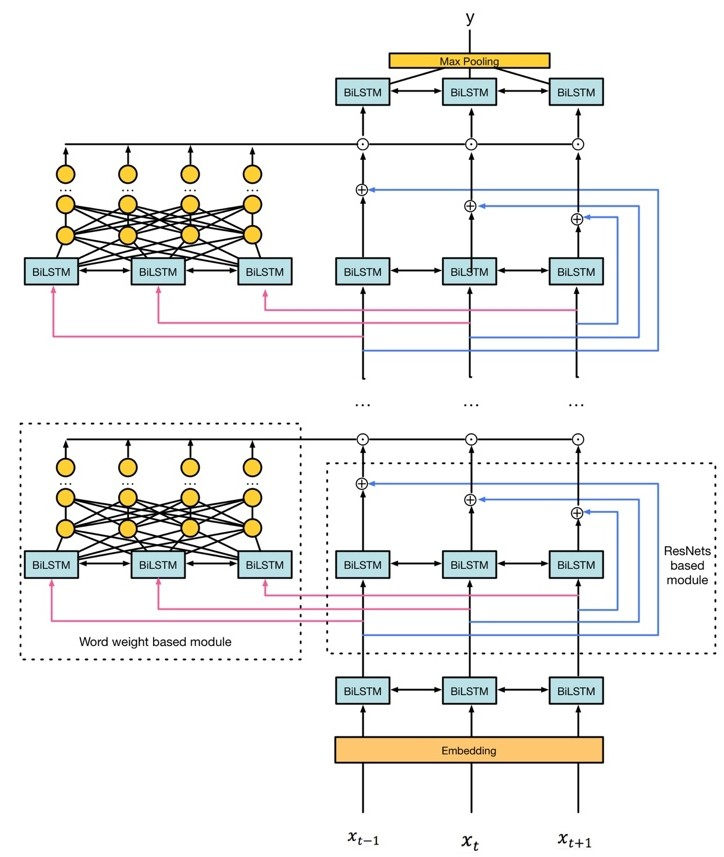
\includegraphics[width=12cm]{model.jpg}\\
  \caption{The instance of Stacked Residual Bi-LSTM with Word Weight Networks. The left line part is the word weight training module and the right part is the ResNets based module.}\label{NBde}
\end{figure}


%%%%%%%%%%%%%%%%%%%%%%%%%%%%%%%%%%%%%%%%%%%%%%%%%%%%%%%%%%%%%%%%%%%%%%%%%%%%%%%



\section{Word weight based module}

Word weight part module has ability to learn the weight of each word. We believe that the word weight is very important in text categorization task, the label of the sentence is often determined by several key words. We focus on constructing this module by using fully connected layers and Bidirectional LSTM (Bi-LSTM)\cite{graves2005framewise} which is the variants of LSTM networks. The standard LSTM is updated as follows:% 
\begin{eqnarray}
i_t &=& \sigma(W_ix_t + U_ih_{t-1} + b_i) \\
f_t &=& \sigma(W_fx_t + U_fh_{t-1} + b_f) \\
\tilde{c}_t &=& tanh(W_cx_t + U_ch_{t-1} + b_c) \\
c_t &=& f_t \odot c_{t-1} + i_t \odot \tilde{c}_t \\
o_t &=& \sigma(W_ox_t + U_oh_{t-1} + b_o) \\
h_t(LSTM) &=& o_t \odot tanh(c_t)
\end{eqnarray}
where $x_t$ are the input of each time step t, $W_j$, $U_j$ are the weight matrices and $b_j$ are the bias vectors, for $j\in \{i,f,c,o\}$. $\sigma$ denotes the sigmoid activation function and $\odot$ denotes element-wise multiplication. The forget gate controls how much of the previous state is going to be thrown away, the input gate controls how much of newly state will be updated, and the output gate controls how much of the internal memory state will be output.

\begin{figure}[t]
  \centering
  % Requires \usepackage{graphicx}
  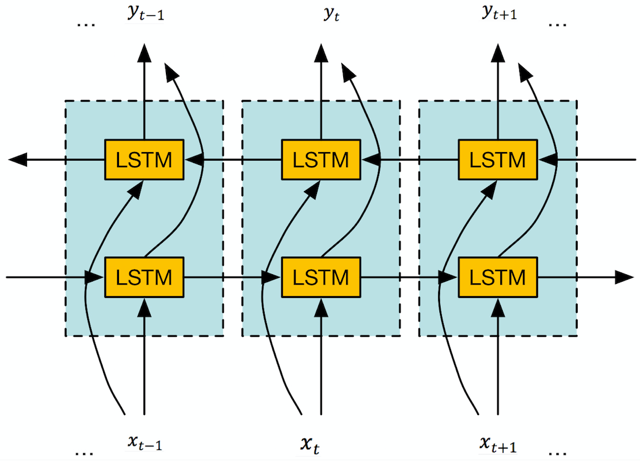
\includegraphics[width=10cm]{bilstm.jpg}\\
  \caption{An illustration of Bidirectional LSTM network.}\label{NBde}
\end{figure}

The Bi-LSTM contains not only the forward $\overrightarrow{LSTM}$ which read the word from the beginning of sentence to the end of sentence but also the backward $\overleftarrow{LSTM}$ which read the word from the end sentence to the beginning of sentence:% 
\begin{eqnarray}
\overrightarrow{h_t} &=& \overrightarrow{h_t(LSTM)} \\
\overleftarrow{h_t} &=& \overleftarrow{h_t(LSTM)} \\
h_{t,Bi-LSTM_W} &=& [\overrightarrow{h_t}, \overleftarrow{h_t}]
\end{eqnarray}
where $h_{t,Bi-LSTM_W}$ is the hidden state of the Bi-LSTM in word weight module which combines the forward and backward hidden states at each time step. Conventional standard LSTMs only utilize previous context with no exploitation of future context, Bi-LSTMs utilize both the previous and future context.

The output of Bi-LSTM will be trained in fully connected layers as the word weight:
\begin{eqnarray}
a_{1,t} &=& h_{t,Bi-LSTM_W} \\
z_{n,t} &=& W_{n-1}a_{n-1,t} + b_{n-1} \\
a_{n,t} &=& ReLU(z_{n,t}) \\
\tilde{W}_t &=& a_{n,t} \\
O_t &=& h_{t,Bi-LSTM_R} \odot \tilde{W}_t
\end{eqnarray}
where $W_{n-1}$ are the weight matrices of fully connected layers, $b_{n-1}$ are the bias vectors, $a_{1,t}$ are the values from input layer of fully connected layers, $a_{n,t}$ are the activation of layer n, $z_{n,t}$ are the total weighted sum of layer n, ReLU\cite{nair2010rectified} is the activation function, $\odot$ is element-wise multiplication, $\tilde{W}_t$ is the word weight of each time step t, $h_{t,Bi-LSTM_R}$ is the hidden state of the Bi-LSTM in right module and $O_t$ are the new hidden state of the Bi-LSTM.\\



%%%%%%%%%%%%%%%%%%%%%%%%%%%%%%%%%%%%%%%%%%%%%%%%%%%%%%%%%%%%%%%%%%%%%%%%%%%%%%%


\section{Residual Networks based module}

\begin{figure}[t]
  \centering
  % Requires \usepackage{graphicx}
  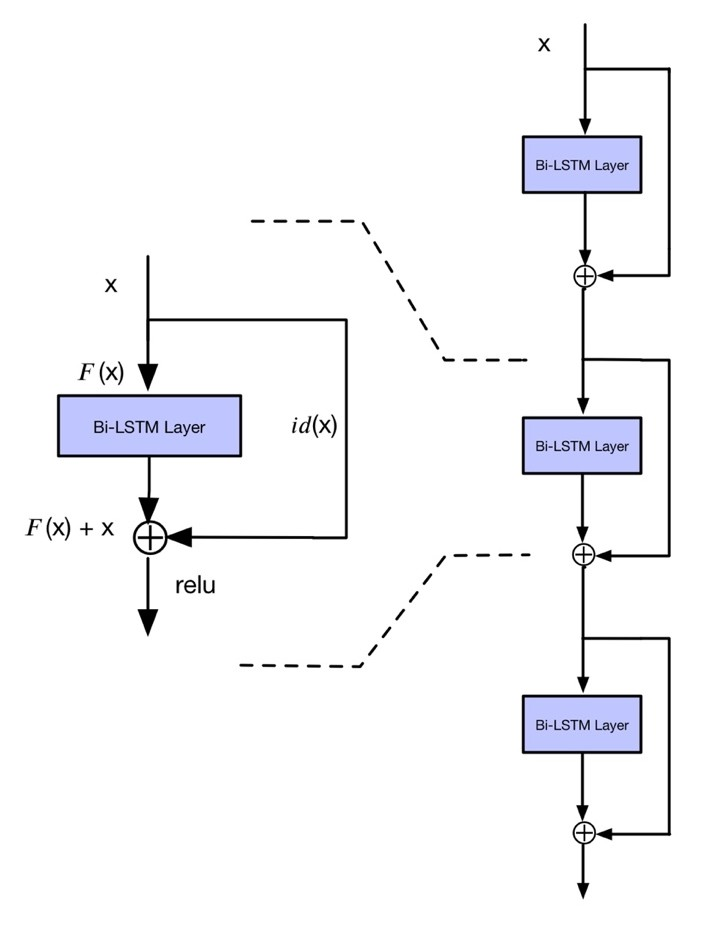
\includegraphics[width=10cm]{resnets.jpg}\\
  \caption{The left image is a residual block in Residual Networks. The right image is an illustration of Residual Networks.}\label{NBde}
\end{figure}

The right part in Figure 3.1 shows the residual part of the model. As we can see, at each layer, the input of Bi-LSTM and the output of Bi-LSTM can be summed directly. The notion of Residual Networks (ResNets) was first introduced by \cite{he2015deep} in image recognition area. The main idea of Residual Networks is to connect some of the layers with shortcuts, which can avoid vanishing gradients and exploding gradients problems, these problems may happen in very deep networks. With the increasing depth of networks, ResNets can improves the accuracy of deep networks.

The shortcut connections have the ability to explicitly let these layers fit a residual mapping with the help of identity transformation. The residual block defined as:
\begin{eqnarray}
&&\mathbb{F}(x_{i-1,t}) = O_t \\
&&x_{i,t} = ReLU(\mathbb{F}(x_{i-1,t}) + id(x_{i-1,t}))
\end{eqnarray}
where $\mathbb{F}(\cdot)$ function represents the Bi-LSTM transformation from $x_{i-1,t}$ layer to $x_{i,t}$ at each time step t, $id(\cdot)$ is an identity mapping function. $ReLU$ is the activation function for output of residual block. 

Although the derivation of Residual Networks is from image recognition area, inspired by its special architecture, we introduce it in our Stacked Bidirectional LSTM when the layers of Stacked Bi-LSTM are deep. The gradients and features which were learned in lower layers can passe through by the identity transformations $id(\cdot)$ in Residual Networks.



%%%%%%%%%%%%%%%%%%%%%%%%%%%%%%%%%%%%%%%%%%%%%%%%%%%%%%%%%%%%%%%%%%%%%%%%%%%%%%%

\begin{figure}[t]
  \centering
  % Requires \usepackage{graphicx}
  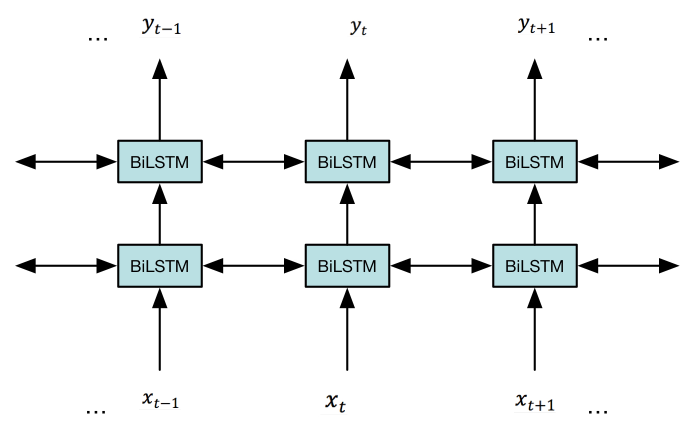
\includegraphics[width=10cm]{stacked.png}\\
  \caption{Stacked structure of Bidirectional LSTM network.}\label{NBde}
\end{figure}

\section{Stacked Residual Bi-LSTM with Word Weight model}

Then, we extend our model to stacked one. Stacked based Bi-LSTM is the vertical multi-layer structure, the output of the lower layer will be the input of the upper layer. By using the stacked based structure, it is possible to achieve different levels of deep abstraction. There are some researches show that the deep hierarchical LSTM based model can be more efficient in representing some functions than a shallow one \cite{graves2013speech}\cite{chung2015gated}.

Finally, the max-pooling of output of Bi-LSTM can be used as the representation of the sentence which can be utilized as the features for text classification.

\begin{figure}[t]
  \centering
  % Requires \usepackage{graphicx}
  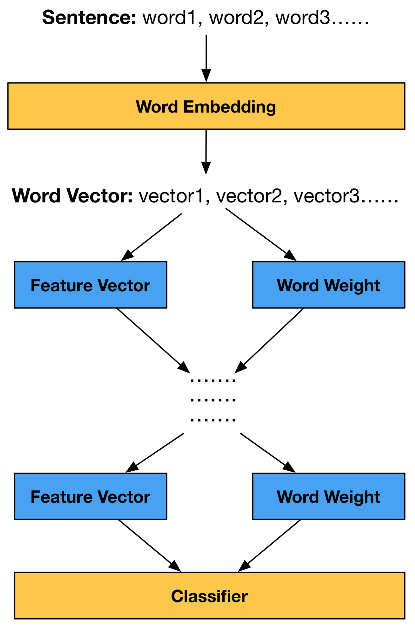
\includegraphics[width=10cm]{workflow.png}\\
  \caption{Work flow of Stacked Residual Bi-LSTM with Word Weight Networks.}\label{NBde}
\end{figure}



The target of the model is to predict label $\hat{y}_j^{(i)}$ for each sentence. We apply cross entropy error function. We train the model over the training examples by minimizing loss of the predicted:
\begin{equation}
L(w) =  \sum_{i=1}^m\sum_{k=1}^K1\{y^{(i)}=k\}log(\hat{y}_j^{(i)})
\end{equation}
where $1{\cdot}$ is indicator function so that 1{true}=1, and 1{false}=0. m is the number of training examples. $y^{(i)}\in \{1,2,\dots K\}$ is true label of each sentence and K is the number of possible labels. $\hat{y}_j^{(i)}\in [0,1]$ is estimated probabilities of each sentence of each label.
	
We use Adam\cite{kingma2014adam} stochastic gradient descent optimizer to update the parameters.



%%%%%%%%%%%%%%%%%%%%%%%%%%%%%%%%%%%%%%%%%%%%%%%%%%%%%%%%%%%%%%%%%%%%%%%%%%%%%%%


\chapter{Experimental Setup}
\section{Datasets}

To show the effectiveness of our model, we choose three different text classification tasks to evaluate our Stacked Residual with Word Weight architectures.

\subsection{Sentiment Classification}
\subsection*{$\bullet$ SST-1}

\begin{table}[t]
\renewcommand{\arraystretch}{1.2}
\caption{The statistical detail of three datasets in our evaluation.}
\label{outcome}
\begin{center}
\begin{tabular}{|c|c|c|c|c|c|c|c|}
\hline
\multicolumn{1}{|c|}{Dataset}
&\multicolumn{1}{c|}{Class}
&\multicolumn{1}{c|}{Train Size}
&\multicolumn{1}{c|}{Valid Size}
&\multicolumn{1}{c|}{Test Size}
&\multicolumn{1}{c|}{Average Length}
&\multicolumn{1}{c|}{Max Length}
&\multicolumn{1}{c|}{Vocabulary Size}\\
\hline
SST-1	&	5	&	8544		&	1101		&	2210		&	19.1		&	56		&	19.5k\\	\hline
SST-2	&	2	&	6920		&	872		&	1821		&	19.3		&	56		&	17.5k\\	\hline
TREC		&	6	&	5452		&	-		&	500		&	9.9		&	37		&	8.9k\\	\hline
\end{tabular}
\end{center}
\label{result1}
\end{table}

The movie reviews consist of 11855 movie reviews with five labels: very negative, negative, neutral, positive, and very positive in Stanford Sentiment Treebank\cite{socher2013recursive}. The dataset is spited into train (8544), dev (1101), and test (2210) for the fine-grained classification task. 

\subsection*{$\bullet$ SST-2}

The movie reviews with binary labels by removing neural labels from the Stanford Sentiment Treebank. The dataset is spited into train (6920), dev (872), and test (1821) for the binary classification task.

\subsection{Question type Classification}
\subsection*{$\bullet$ TREC}

We choose the TREC\cite{li2002learning} which is a question type classification benchmark. TREC consists of 6 classes, including location, human, entity, abbreviation, description and numeric. The training dataset contains train (5452) and test (500) questions.



%%%%%%%%%%%%%%%%%%%%%%%%%%%%%%%%%%%%%%%%%%%%%%%%%%%%%%%%%%%%%%%%%%%%%%%%%%%%%%%



\section{BaseLines}

We compare our model with several models as follow:

$\bullet$ \textbf{SVM} SVM with unigram and bigram features.

$\bullet$ \textbf{NBOW} NBoW averages word vectors and applies a softmax classification layer.

$\bullet$ \textbf{Paragraph Vector} Paragraph Vector learns fixed-length feature representations from variable-length pieces of texts.

$\bullet$ \textbf{CNN-non-static} Convolutional Neural Network based model with fine-tuned word vectors\cite{kim2014convolutional}.

$\bullet$ \textbf{CNN-multichannel} Convolutional Neural Network based model with multi-channels\cite{kim2014convolutional}.

$\bullet$ \textbf{DCNN} Dynamic Convolutional Neural Network with dynamic k-max pooling\cite{kalchbrenner2014convolutional}.

$\bullet$ \textbf{RAE} Recursive autoencoder\cite{socher2013recursive}.

$\bullet$ \textbf{MV-RNN} Matrix-Vector Recursive Neural Network\cite{socher2013recursive}.

$\bullet$ \textbf{RNTN} Tensor based Recursive Neural Tensor Network\cite{socher2013recursive}.

$\bullet$ \textbf{DRNN} Multi-layer stacked Recursive Neural Network\cite{irsoy2014deep}.

$\bullet$ \textbf{MTL-RNN} A multi-task learning framework to jointly learn across multiple related tasks\cite{liu2016recurrent}.

$\bullet$ \textbf{Tree-LSTM} A LSTMs to tree-structured network topologies\cite{tai2015improved}.

$\bullet$ \textbf{C-LSTM} Unified Model which utilizes CNN and LSTM\cite{zhou2015c}.


%%%%%%%%%%%%%%%%%%%%%%%%%%%%%%%%%%%%%%%%%%%%%%%%%%%%%%%%%%%%%%%%%%%%%%%%%%%%%%%


\section{Hyperparameters and Training}

In our experiments, we initialize word embeddings with the publicly available 300-dimensional word vectors. The vectors are pre-trained with word2vec on Google News Dataset which contains about 100B words. We also initialize the vector with the uniform distribution [-0.25, 0.25] for words which are not in word2vec vectors.

\begin{table}[t]
\renewcommand{\arraystretch}{0.8}
\caption{Some other hyperparameters settings among three datasets.}
\label{outcome}
\begin{center}
\begin{tabular}{|c|c|c|}
\hline
\multicolumn{1}{|c|}{Hyperparameters}
&\multicolumn{1}{c|}{SST-1/SST-2}
&\multicolumn{1}{c|}{TREC}\\
\hline
\begin{tabular}[x]{@{}c@{}}Memory dimension\\(Bi-LSTM)\end{tabular}	&	150	&	300	\\	\hline
\begin{tabular}[x]{@{}c@{}}Stacked layers\\(Residual part)\end{tabular}	&	10	&	5	\\	\hline
\begin{tabular}[x]{@{}c@{}}FC hidden layers\\(Each weight part)\end{tabular}	&	5	&	5	\\	\hline
\begin{tabular}[x]{@{}c@{}}FC hidden layers\\(Each weight part)\end{tabular}	&	50	&	50	\\	\hline
\end{tabular}
\end{center}
\label{result1}
\end{table}

We train our model with Adam stochastic gradient descent optimizer with a learning rate of 0.001 and we use a mini-batch size of 50. The parameters are initialized from uniform distribution in [-0.1, 0.1]. The parameters were regularized with L2 regularization with factor of $10^{-4}$. We also apply dropout\cite{hinton2012improving} with a probability of 0.5 on both weight part and residual part of model during the training to prevent overfitting.

Other hyperparameters settings are shown in Table 4.2, for SST, the LSTM dimension is 150, so the combination of forward and backward in Bi-LSTM is 300 dimensions for output vector. The same as TREC.




%%%%%%%%%%%%%%%%%%%%%%%%%%%%%%%%%%%%%%%%%%%%%%%%%%%%%%%%%%%%%%%%%%%%%%%%%%%%%%%



\section{Results and Analysis}
\subsection{Text classification}

\begin{table}[t]
\renewcommand{\arraystretch}{1.1}
\caption{Classification accuracy of our method compared with other models on three datasets.}
\label{outcome}
\begin{center}
\begin{tabular}{|c|c|c|c|c|}
\hline
\multicolumn{1}{|c|}{}
&\multicolumn{1}{c|}{Methods}
&\multicolumn{1}{c|}{SST-1}
&\multicolumn{1}{c|}{SST-2}
&\multicolumn{1}{c|}{TREC}\\
\hline
\begin{tabular}[x]{@{}c@{}}Socher et al., 2013(a)\\Silva et al., 2011(b)\end{tabular}	& SVM & 40.7\%(a) & 79.4\%(a) & 95\%(b)		\\	\hline
Kalchbrenner et al., 2014 & NBOW & 42.4\% & 80.5\% & -	\\	\hline
\begin{tabular}[x]{@{}c@{}}Le and Mikolov, 2014(a)\\Zhao et al., 2015(b)\end{tabular}	& Paragraph Vector & 48.7\%(a) & 87.8\%(a) & 91.8\%(b)		\\	\hline
Kim, 2014 & CNN-non-static & 48.0\% & 87.2\% & 93.6\%	\\	\hline
Kim, 2014 & CNN-multichannel & 47.4\% & 88.1\% & 92.2\%	\\	\hline
Kalchbrenner et al., 2014 & DCNN & 48.5\% & 86.8\% & 93.0\%	\\	\hline
Socher et al., 2013 & RAE & 43.2\% & 82.4\% & -	\\	\hline
Socher et al., 2013 & MV-RNN & 44.4\% & 82.9\% & -	\\	\hline
Socher et al., 2013 & RNTN & 45.7\% & 85.4\% & -	\\	\hline
Irsoy aet al., 2014 & DRNN & 49.8\% & 86.6\% & -	\\	\hline
Liu et al.,2016 & MTL-RNN & 49.6\% & 87.9\% & -	\\	\hline
Tai et al., 2015 & Tree-LSTM & 51.0\% & 88.0\% & -	\\	\hline
Zhou et al.,2015 & C-LSTM & 49.2\% & 87.8\% & 94.6\%	\\	\hline
 \textbf{This paper} &  \textbf{SRW-RNN} &  \textbf{52.7\%} &  \textbf{88.2\%} &  \textbf{94.7\%}	\\	\hline
\end{tabular}
\end{center}
\label{result1}
\end{table}

The experimental results are showed in Table 4.3. We compare our model with a variety of models, the Stacked Residual with Word Weight structure model has high performance on text classification task without any additional feature engineering.

Fore SST datasets, our proposed method outperforms existing models and achieves state-of-art prediction accuracy on both fine-grained classification task and binary classification task of Stanford Sentiment Treebank. In particular, our model obtains 52.7\% classification accuracy on fine-grained classification task which is a very substantial improvement. For TREC, our result is close to the best result. Although we did not beat the state-of-the-art one, comparing with Stanford Sentiment Treebank, we find that not only the average sentence’s length of SST is longer than TREC, but also the Semantic complexity of SST is much more complicated than TREC. Through the analysis, we find that our model is applicable to the semantics of complex sentence which can learn more features from sentences. The Stacked Residual with Word Weight structure can learn the weight of different words in the sentence during the training, it is very useful for sentence representation that can increase the prediction accuracy. 

In summary, the results mean that our model can extract more information and learn high hierarchical features from the text than others methods on dataset which has complex semantics.





\subsection{Model Analysis}
Benefiting from the word weight structure, our model can learn the importance of different words very well, each word has its own weight which is the high potential features in a sentence. Most of the time, the label of each sentence is determined by several key words, and word weight part can capture these key words easily.

As we can see from Figure 4.1 (a), comparing with the standard stacked Bi-LSTM without residual part, during the training step, the convergence speed of our model is faster. The inputs of a lower layer in stacked Bi-LSTM are made available to a node in a higher layer because of the shortcut connections which can lead the network easy trained.

The Figure 4.1 (b) shows the test accuracy between two models. this figure indicates that the residual structure has ability to achieve high accuracy and the gradients can easily back propagate through them, which results in a faster converging.

\begin{figure}[t]
  \centering
  % Requires \usepackage{graphicx}
  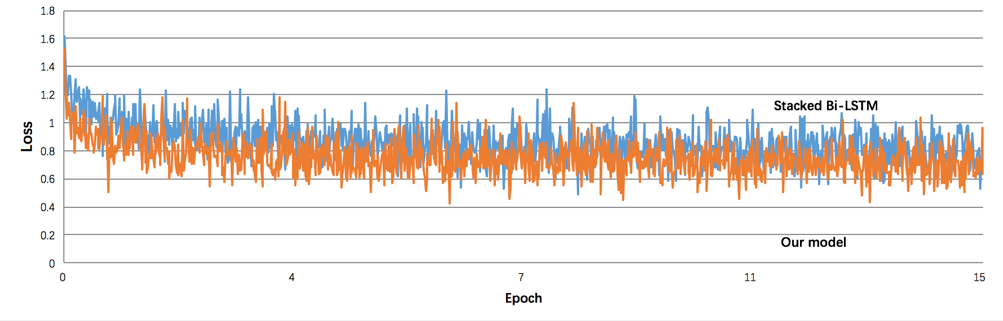
\includegraphics[width=16cm]{result_1.png}\\
  {(a)}\\
  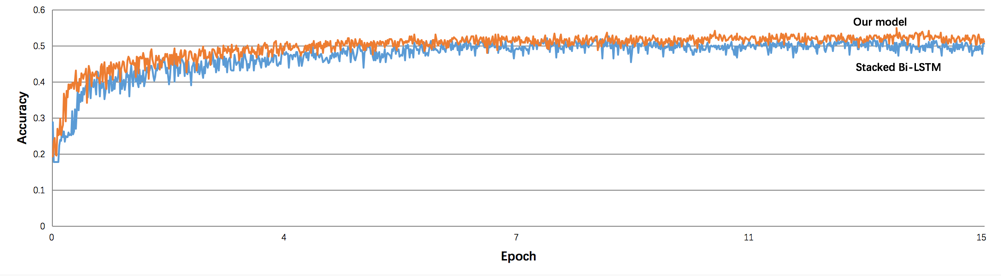
\includegraphics[width=16cm]{result_2.png}\\
  {(b)}\\
  \caption{The (a) shows the batch training loss on SST-1 with our method and standard stacked Bi-LSTM. The (b) shows the test accuracy on SST-1 compared with two methods.}\label{NBde}
\end{figure}




\chapter{Conclusions}

In this paper, we introduce a novel text classification model called Stacked Residual Recurrent Neural Network with word weight. This model is able to extract more features and learn high hierarchical meaning of each word in a sentence. It also can identify the importance of different words due to its word weight structure. The residual structure makes model more expressive when stacked layers are deep. Experimental results show that our model can achieve high performance on text classification task than any other methods. This suggests our model can capture more potential features in sentences.







\bibliographystyle{IEEEtran}
\bibliography{LUOreference}


\end{document}
